\section{Paired audit of Pearson-bootstrap calibration}\label{sec:audit}
The original diagnostic uses fixed bootstrap standard deviations for local Fisher-z Pearson differences. It showed substantial undercoverage in some IID and serially dependent cells. To identify which features matter, the new audit holds datasets fixed and varies bootstrap mechanism, studentizer and resample count.

Three IID Gaussian independence cells, $(p,n)=(12,252),(52,252),(52,1008)$, each contain 1,000 datasets. We compare the original row bootstrap with 499 and 1,999 resamples, an IID row bootstrap with empirical influence standard deviations and 1,999 resamples, and Gaussian influence multipliers with 1,999 draws. The 499 row draws are nested in the 1,999 draws. For Pearson correlation, standardized observations $z_{ti}$ give influence
\[
 \phi_{t,ij}=\frac{z_{ti}z_{tj}-\widehat\rho_{ij}(z_{ti}^2+z_{tj}^2)/2}{1-\widehat\rho_{ij}^2}.
\]
We centre these influences across rows and use $n^{-2}\sum_t(\phi_{te}-\phi_{tf})^2$ for a contrast variance. Every calibration uses the same local family, Fisher-z estimand and maximum statistic. Under independence, every population contrast is zero, making input undercoverage identical to any false strict order. We report paired differences between procedures, not just isolated estimates.

Direct index resampling checks the count-weighted covariance implementation. Independent calculations check influences, studentizers and maxima. This audit evaluates particular procedures at these sample sizes; it separates an implementation check from a conclusion about bootstrap calibration. The earlier 24-cell diagnostic, including serial dependence, is retained in the reproducibility materials.

\begin{table}[htbp]\centering\small
\setlength{\tabcolsep}{4pt}
\caption{Paired Gaussian IID null audit. Each procedure uses the same 1,000 datasets in a cell; 499 row draws are nested in 1,999. FWER equals input undercoverage in this all-ties population. Intervals are individual Wilson Monte Carlo intervals.}\label{tab:audit}
\begin{lrbox}{\resultsbox}\begin{tabular}{llrr}
\toprule
$p$, $n$ & Calibration, studentizer, $B$ & FWER & 95\% MC interval\\
\midrule
12, 252 & Row, bootstrap SD, 499 & 0.098 & [0.081, 0.118]\\
12, 252 & Row, bootstrap SD, 1999 & 0.088 & [0.072, 0.107]\\
12, 252 & Row, influence SD, 1999 & 0.085 & [0.069, 0.104]\\
12, 252 & Gaussian, influence SD, 1999 & 0.097 & [0.080, 0.117]\\
52, 252 & Row, bootstrap SD, 499 & 0.215 & [0.191, 0.242]\\
52, 252 & Row, bootstrap SD, 1999 & 0.162 & [0.140, 0.186]\\
52, 252 & Row, influence SD, 1999 & 0.152 & [0.131, 0.176]\\
52, 252 & Gaussian, influence SD, 1999 & 0.188 & [0.165, 0.213]\\
52, 1008 & Row, bootstrap SD, 499 & 0.107 & [0.089, 0.128]\\
52, 1008 & Row, bootstrap SD, 1999 & 0.086 & [0.070, 0.105]\\
52, 1008 & Row, influence SD, 1999 & 0.067 & [0.053, 0.084]\\
52, 1008 & Gaussian, influence SD, 1999 & 0.076 & [0.061, 0.094]\\
\bottomrule\end{tabular}\end{lrbox}\ifdim\wd\resultsbox>\linewidth\resizebox{\linewidth}{!}{\usebox{\resultsbox}}\else\usebox{\resultsbox}\fi\end{table}
At $p=52,n=1008$, the paired FWER difference (499 minus 1,999 row draws with the original studentizer) is 0.021, with Monte Carlo interval [0.007,0.035] based on paired replication differences. The studentizer and mechanism comparisons in Table~\ref{tab:audit} provide separate diagnostics. The verified resampling identities support implementation correctness; the calibration results concern the particular finite-sample procedures.
\begin{figure}[htbp]\centering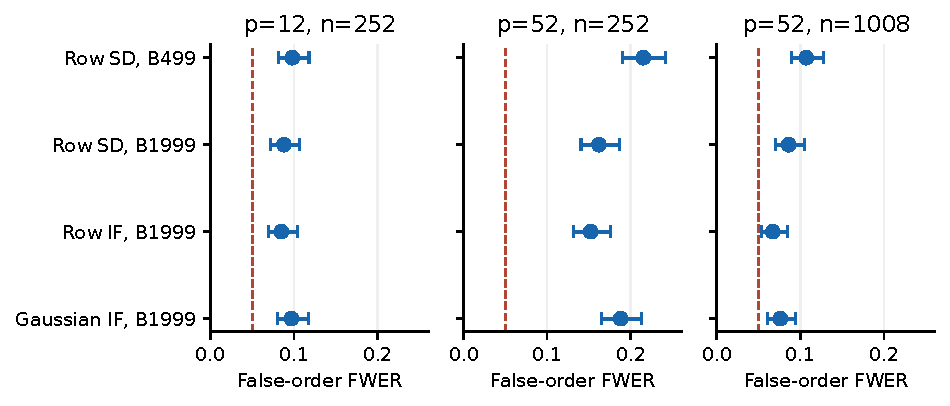
\includegraphics[width=\textwidth]{Fig_audit.pdf}
\caption{False-order FWER in the paired IID audit. Horizontal intervals are individual Wilson Monte Carlo intervals; the vertical line marks 0.05.}\label{fig:audit}\end{figure}


